\documentclass[12pt, a4paper]{article}
% --- Codificación y lenguaje ---
\usepackage[utf8]{inputenc}
\usepackage[T1]{fontenc}
\usepackage[spanish]{babel}

% --- Márgenes ---
\usepackage[top=2.5cm, bottom=2.5cm, left=3cm, right=2.5cm]{geometry}

% --- Tipografía ---
\usepackage{lmodern}

% --- Matemáticas ---
\usepackage{amsmath}
\usepackage{amssymb}

% --- Figuras y tablas ---
\usepackage{graphicx}
\usepackage{booktabs}
\usepackage{float}
\usepackage{caption}
\usepackage{subcaption}

% --- Colores ---
\usepackage{xcolor}

% --- Hipervínculos ---
\usepackage[colorlinks=true, linkcolor=blue, citecolor=blue, urlcolor=blue]{hyperref}

% --- Interlineado ---
\usepackage{setspace}
\onehalfspacing

% --- Encabezados y pies de página ---
\usepackage{fancyhdr}
\pagestyle{fancy}
\fancyhf{}
\lhead{\small Región Andina occidental (1996--2025)}
\rhead{\small Mini Proyecto 2}
\rfoot{\thepage}

% --- Bibliografía ---
\usepackage[numbers, sort&compress]{natbib}

% =============================================================
\begin{document}
	
	\begin{titlepage}
		\centering
		\vspace*{2cm}
		{\LARGE \textbf{Mini Proyecto 3: Equilibrio Radiativo-Convectivo y Convección Organizada en los Trópicos}\\[0.5em]
			\large Réplica observacional de Jakob et al. (2019)\\
			\textit{Journal of Geophysical Research: Atmospheres}}\\[2cm]
		{\large Jhon García Barrera}\\[0.5em]
		{\normalsize Física del Clima y Cambio Climático}\\[0.5em]
		{\normalsize \today}\\[3cm]
		\vfill
		{\small Código y datos disponibles en:\\
			\url{https://github.com/jhongarciab/proyectos-clima/tree/main/proyecto%203}}
	\end{titlepage}
	
	\tableofcontents
	\newpage

\section{Resumen del Paper}

\subsection{Contexto y motivación}

El equilibrio radiativo-convectivo (RCE, por sus siglas en inglés) describe un estado de balance entre el enfriamiento de la atmósfera por radiación y el calentamiento producido por la liberación de calor latente en la precipitación y por los flujos de calor sensible desde la superficie. Si bien el RCE constituye una restricción energética bien establecida a escala global, se sabe poco sobre la proximidad de la atmósfera tropical real a este estado en escalas espaciales y temporales más pequeñas, a pesar de su uso frecuente en estudios de modelado idealizados. Esta brecha de conocimiento motiva el trabajo de \cite{jakob2019rce}, que proporciona la primera evaluación observacional de las escalas a las que la atmósfera tropical se encuentra cerca del RCE.

El estudio responde tres preguntas fundamentales:
\begin{enumerate}
	\item ¿A qué escalas espaciales y temporales se encuentra la atmósfera tropical cerca del RCE?
	\item ¿Cómo contribuyen las diferentes regiones tropicales al RCE a escala global?
	\item Cuando la atmósfera está en RCE, ¿qué papel juega la convección organizada en su mantenimiento?
\end{enumerate}

Para evaluar la proximidad al RCE, los autores calculan el balance termodinámico del presupuesto de energía de la atmósfera integrado verticalmente. En ausencia de cambios en el contenido de calor local y de divergencia del flujo de energía estática seca, el RCE requiere que se cumpla:

\begin{equation}
	D_{\text{RCE}} = LP + Q_R + H \approx 0
\end{equation}

\noindent donde $LP$ es el calentamiento latente por precipitación, $Q_R$ es el enfriamiento radiativo atmosférico y $H$ es el flujo de calor sensible superficial. Se define un estado cercano al RCE como aquel en que $|D_{\text{RCE}}| < 50\,\text{W\,m}^{-2}$, un umbral que reconoce la incertidumbre observacional y la imposibilidad de un balance exacto salvo en promedios globales de largo plazo.

Los datos utilizados cubren el período 2001--2009 y provienen de cuatro fuentes:

\begin{itemize}
	\item \textbf{CERES SYN1deg Ed4a}: estimaciones diarias de flujos radiativos en TOA y superficie a resolución $1^\circ \times 1^\circ$, usadas para calcular $Q_R = R_{\text{TOA,net}} - R_{\text{SFC,net}}$.
	\item \textbf{GPCP 1DD v1.2}: precipitación diaria a resolución $1^\circ \times 1^\circ$, convertida a unidades de flujo energético mediante $P_E \approx L \times P / 86{,}400$.
	\item \textbf{Reanálisis NCEP}: flujo de calor sensible superficial ($H$) y movimiento vertical a 500~hPa ($\omega$), en grilla de $2.5^\circ \times 2.5^\circ$.
	\item \textbf{ISCCP D1}: regímenes de nubes derivados del análisis de histogramas conjuntos de presión de tope nuboso y espesor óptico en regiones de $280 \times 280$~km.
\end{itemize}

\subsection{Resultados principales}

El promedio de 9 años sobre el dominio tropical completo ($30^\circ$N--$30^\circ$S) arroja
$Q_R = -104.5\,\text{W\,m}^{-2}$, $LP = 85.2\,\text{W\,m}^{-2}$ y $H = 22.6\,\text{W\,m}^{-2}$,
con un desequilibrio de apenas $3.3\,\text{W\,m}^{-2}$, consistente con la idea de que los
trópicos en conjunto están cerca del RCE. Sin embargo, \emph{localmente} la atmósfera tropical
se encuentra muy lejos del equilibrio en casi todas partes. En las regiones precipitantes,
el calentamiento latente supera ampliamente el enfriamiento radiativo, mientras que en las
regiones de subsidencia ocurre lo opuesto.

El histograma bidimensional de $Q_R$ versus $P_E$ en los 22{,}320 puntos de grilla tropicales
revela cinco regiones características: la región~1 (baja precipitación, fuerte enfriamiento)
corresponde a los océanos subtropicales orientales dominados por subsidencia; la región~2
(baja precipitación, débil enfriamiento) representa los desiertos continentales; la región~3
(precipitación intermedia, débil enfriamiento) incluye los bordes exteriores de la ZCIT;
la región~4 (precipitación intermedia, fuerte enfriamiento) agrupa zonas de transición; y
la región~5 (alta precipitación) corresponde al núcleo de la ZCIT. Esta distribución refleja
la naturaleza fuertemente no local del RCE: el equilibrio tropical se alcanza mediante la
compensación entre regiones convectivamente activas y regiones de subsidencia.

\subsection{Dependencia de escala y convección organizada}

La fracción de días en que una región se encuentra cerca del RCE aumenta fuertemente con
la escala espacial de promediado. A escala de $1^\circ \times 1^\circ$, apenas el $\sim$10\%
de los días cumplen la condición $|D_{\text{RCE}}| < 50\,\text{W\,m}^{-2}$, dado que la
precipitación diaria local es altamente intermitente y puede alcanzar valores de hasta
$2{,}000\,\text{W\,m}^{-2}$ ($\approx$70~mm~día$^{-1}$). Para dominios de
$50^\circ \times 50^\circ$ ($\approx$5{,}000~km), más del 80\% de los días son cercanos al
RCE incluso en promedios diarios. Para que una región esté en RCE al menos el 80\% del tiempo
se requieren dominios de al menos $5{,}000 \times 5{,}000$~km$^2$. El promediado temporal tiene
un efecto secundario respecto al espacial: pasar de promedios diarios a promedios de 5 o
10~días incrementa la frecuencia de RCE en apenas $\sim$10\%, mientras que el promediado
espacial produce aumentos mucho más pronunciados. Se observa además un comportamiento no
monótono con la escala, con un mínimo local en torno a $20^\circ$, reflejo de que a esa
escala la región comienza a incluir simultáneamente las bandas de lluvia de la ZCIT y la
SPCZ al norte y sur del ecuador.

Mediante los regímenes de nubes del ISCCP~D1, los autores muestran que cuando la atmósfera
está en RCE a escala de $20^\circ \times 20^\circ$, predominan los estados de nubes suprimidas
(régimen ST, $\sim$45\%) y cirros delgados (régimen IC, $\sim$25\%), mientras que la
convección profunda organizada (régimen CD) ocurre apenas el 5\% del tiempo. La convección
organizada es esencialmente ausente cuando dominios pequeños
($< 1{,}000 \times 1{,}000$~km$^2$) están en RCE, y a escalas mayores su fracción permanece
constante mientras los estados suprimidos dominan la mezcla. Esto indica que el RCE se logra
mediante una combinación de una pequeña área de convección activa intensa y grandes áreas
de subsidencia, no mediante convección organizada predominante.

\subsection{Conclusiones}

Jakob et. al. demuestran que la atmósfera tropical en conjunto se encuentra cerca del
RCE en escala diaria, pero a nivel local está lejos del equilibrio casi en todo momento.
Alcanzar el RCE frecuentemente requiere promediar sobre dominios de varios miles de
kilómetros. El papel de la convección organizada es secundario: su ocurrencia es rara en
estados de RCE. Los desiertos, mediante su escaso calentamiento latente y alto enfriamiento
radiativo, juegan un papel importante en el balance energético tropical global. Estos
resultados cuestionan la relevancia directa de los experimentos de modelado de RCE en
dominios pequeños para representar el comportamiento observado de la atmósfera tropical real.

\section{Resultados}

\subsection{Figura 1}

\begin{figure}[h]
	\centering
	\begin{subfigure}[t]{0.48\textwidth}
		\centering
		\includegraphics[width=\textwidth]{../../figuras/jakob2019_fig01_original.png}
		\caption{Original — Jakob et al. (2019)}
	\end{subfigure}
	\hfill
	\begin{subfigure}[t]{0.46\textwidth}
		\centering
		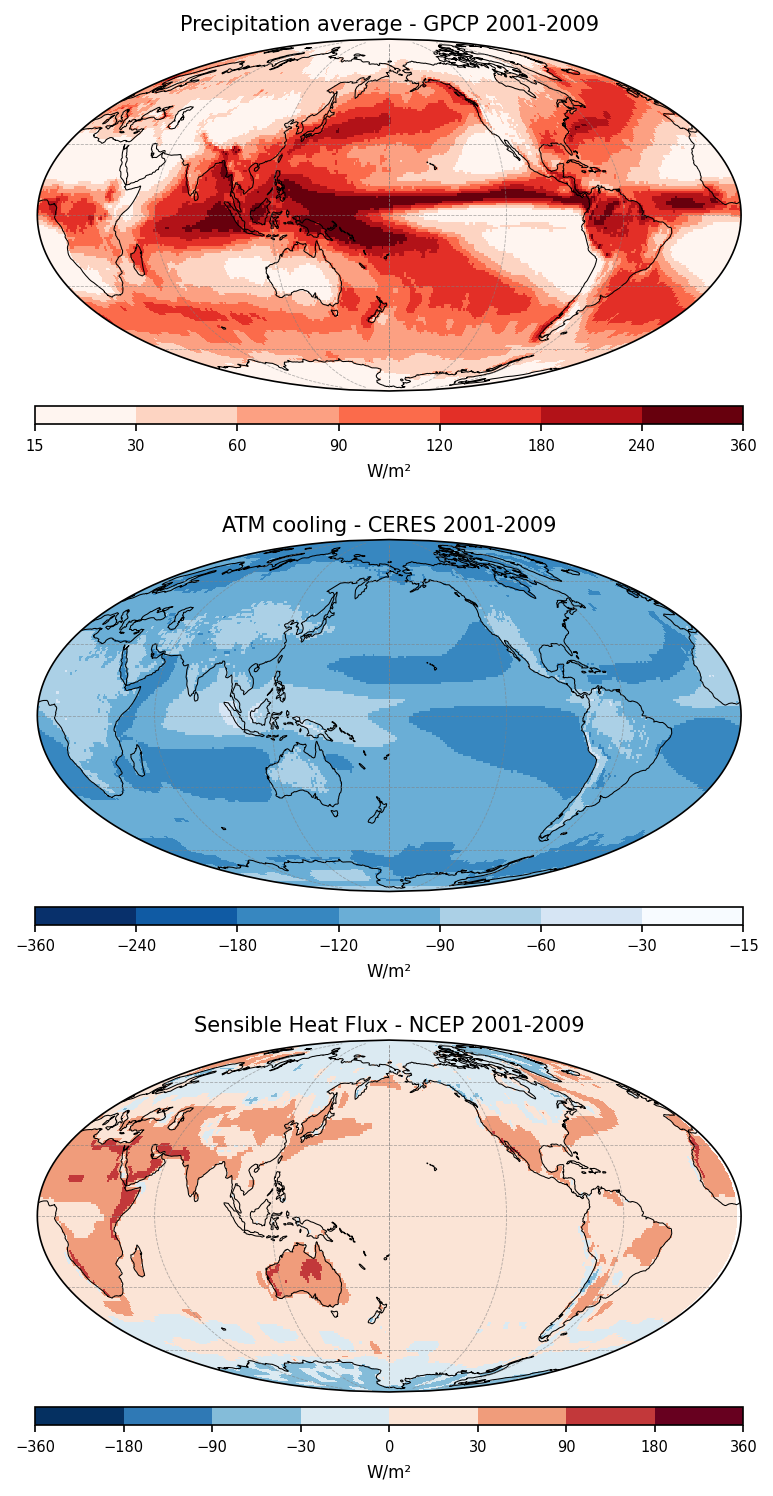
\includegraphics[width=\textwidth]{../../figuras/fig01_jakob2019.png}
		\caption{Réplica}
	\end{subfigure}
	\caption{Promedio de 9 años de la precipitación expresada en unidades de energía
		($P_E$, superior), el enfriamiento radiativo atmosférico ($Q_R$, medio) y el flujo
		de calor sensible superficial ($H$, inferior) para el período 2001--2009.}
	\label{fig:fig01}
\end{figure}

La Figura~\ref{fig:fig01} muestra la distribución espacial global de los tres términos
del balance termodinámico del RCE promediados sobre los 9 años del período de análisis.
La precipitación intensa se concentra en la ZCIT y la SPCZ, con valores que superan los
$240\,\text{W\,m}^{-2}$ en el Pacífico occidental y el Índico tropical. El enfriamiento
radiativo es más intenso sobre los océanos subtropicales orientales y los desiertos
continentales, donde la ausencia de nubes altas permite un enfriamiento eficiente, y más
débil sobre las regiones convectivas activas. El calor sensible es pequeño sobre los
océanos y significativo solo sobre las regiones áridas continentales. La réplica reproduce
fielmente los patrones espaciales del original sin diferencias apreciables.

\subsection{Figura 2}

\begin{figure}[h]
	\centering
	\includegraphics[width=0.85\textwidth]{../../figuras/jakob2019_fig02_original.png}
	\caption*{Original — Jakob et al. (2019)}
	\vspace{0.5cm}
	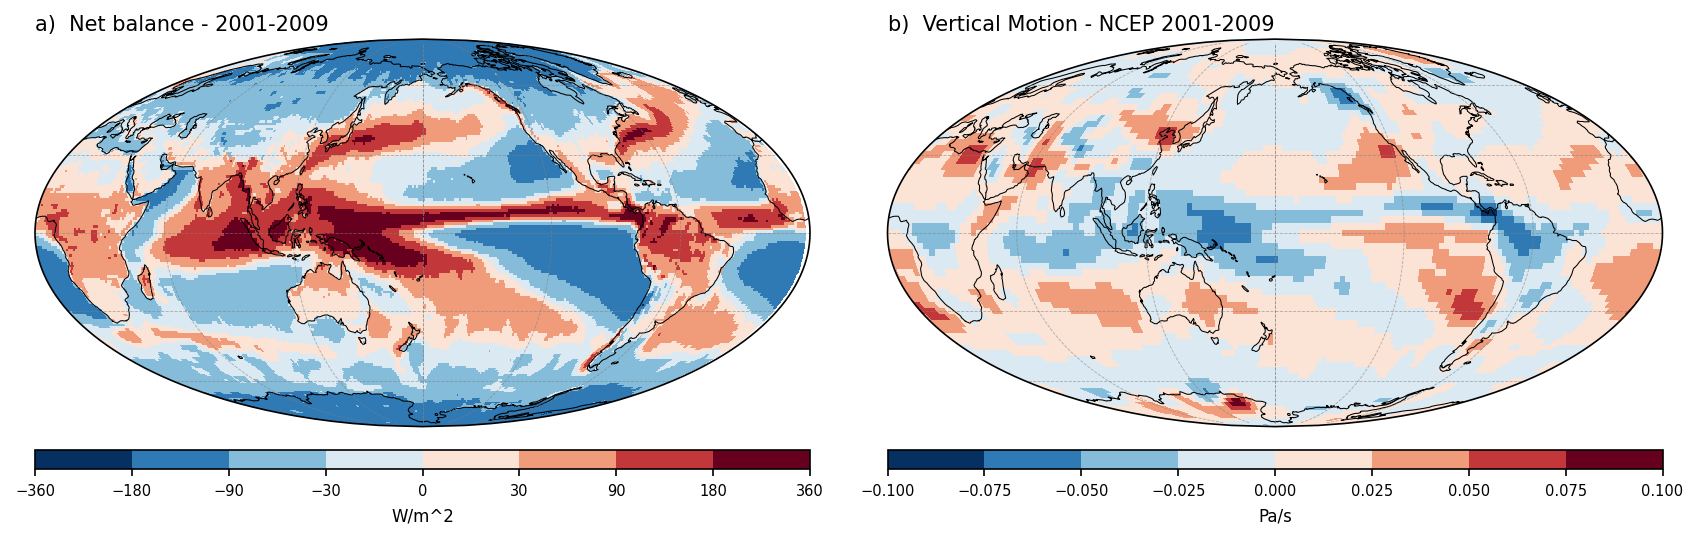
\includegraphics[width=0.85\textwidth]{../../figuras/fig02_jakob2019.png}
	\caption*{Réplica}
	\caption{Promedio de 9 años del balance neto termodinámico $D_{\text{RCE}}$
		(panel a) y del movimiento vertical a 500~hPa (panel b) para el período
		2001--2009. El balance neto combina los tres términos del presupuesto energético
		($Q_R + LP + H$) y el movimiento vertical proviene del reanálisis NCEP.}
	\label{fig:fig02}
\end{figure}

La Figura~\ref{fig:fig02} ilustra la distribución espacial del desequilibrio
termodinámico local y su vínculo con la circulación atmosférica. El panel~(a) muestra
que el balance neto $D_{\text{RCE}}$ es positivo en las regiones convectivas activas
(ZCIT y SPCZ), donde el calentamiento latente supera ampliamente el enfriamiento
radiativo, y negativo en las regiones de subsidencia subtropical y los desiertos,
donde el enfriamiento radiativo domina. El panel~(b) confirma que las regiones de
desequilibrio positivo están asociadas con movimiento vertical ascendente (omega
negativo), mientras que las de desequilibrio negativo corresponden a subsidencia
(omega positivo), evidenciando el papel de la circulación dinámica en mantener a la
atmósfera local alejada del RCE a lo largo del tiempo.

La réplica reproduce fielmente los patrones espaciales del original en ambos paneles.
El panel~(b) presenta celdas visualmente más grandes debido a la resolución nativa
de $2.5^\circ \times 2.5^\circ$ del reanálisis NCEP~1, idéntica a la usada por
\cite{jakob2019rce}.

\subsection{Figura 3}

\begin{figure}[h]
	\centering
	\begin{subfigure}[t]{0.52\textwidth}
		\centering
		\includegraphics[width=\textwidth]{../../figuras/jakob2019_fig03_original.png}
		\caption*{Original — Jakob et al. (2019)}
	\end{subfigure}
	\hfill
	\begin{subfigure}[t]{0.44\textwidth}
		\centering
		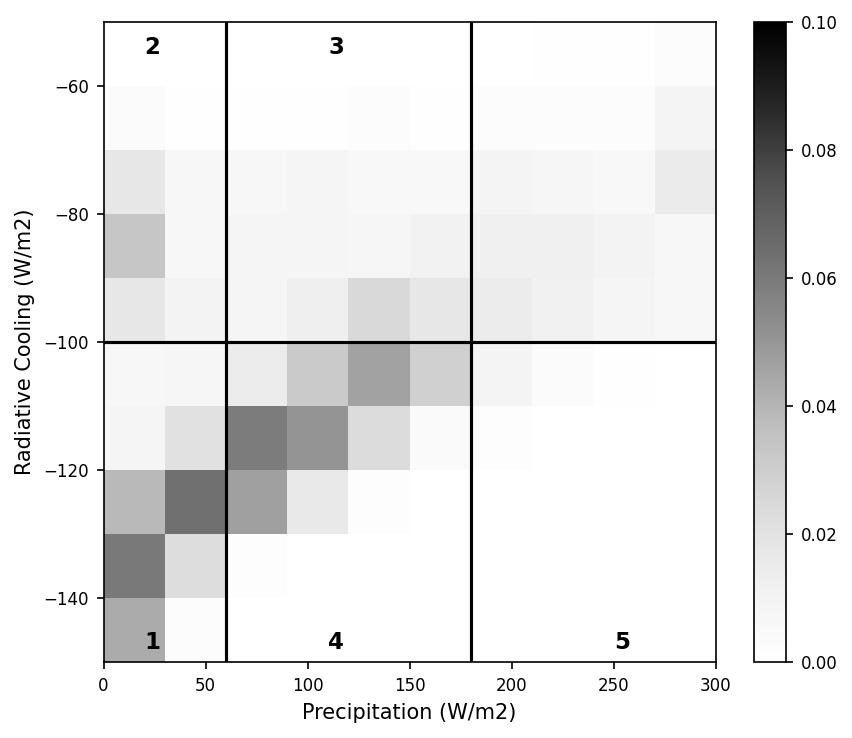
\includegraphics[width=\textwidth]{../../figuras/fig03_jakob2019.png}
		\caption*{Réplica}
	\end{subfigure}
	\caption{Histograma bidimensional de la frecuencia relativa de ocurrencia de
		combinaciones de precipitación media de 9 años en unidades de energía ($P_E$)
		y enfriamiento radiativo ($Q_R$) en los puntos de grilla tropicales. Las líneas
		negras delimitan las cinco regiones características del histograma. El número
		total de puntos de grilla es 22{,}320.}
	\label{fig:fig03}
\end{figure}

La Figura~\ref{fig:fig03} muestra la distribución conjunta de $P_E$ y $Q_R$ en los
22{,}320 puntos de grilla tropicales ($30^\circ$S--$30^\circ$N) a partir de los
promedios de 9 años. La gran mayoría de los puntos presenta poco o ningún calentamiento
latente acompañado de fuerte enfriamiento radiativo (región~1), correspondiente a los
océanos subtropicales y desiertos donde la subsidencia domina. El segundo grupo más
poblado es de precipitación intermedia con enfriamiento significativo (región~3). La
anticorrelación entre precipitación alta y enfriamiento fuerte en la región~5 confirma
que el RCE es un fenómeno de escala no local: cuando llueve intensamente, las nubes
altas asociadas reducen la eficiencia del enfriamiento radiativo.

La réplica presenta dos diferencias respecto al original, ambas atribuibles al uso de
GPCP~v3.3 en lugar de v1.2. En primer lugar, la distribución está desplazada hacia la
derecha en el eje $P_E$: la media tropical de $P_E$ en nuestra réplica es de
$100.8\,\text{W\,m}^{-2}$ frente a $85.2\,\text{W\,m}^{-2}$ del paper, una diferencia
de $\sim$18\% derivada del algoritmo GPM~IMERG incorporado en v3.3, que captura mejor
los eventos convectivos intensos. En segundo lugar, las celdas más oscuras del
histograma no alcanzan la saturación visual del original: dado que la densidad se
distribuye sobre un rango más amplio de $P_E$, ninguna celda individual acumula la
fracción de frecuencia suficiente para aparecer completamente negra. Ambas diferencias
son sistemáticas y consistentes con la versión de datos utilizada; los patrones
cualitativos ---la concentración en bajas precipitaciones, la anticorrelación a altas
precipitaciones y la estructura de cinco regiones--- se reproducen correctamente.

\subsection{Figura 4}

\begin{figure}[h]
	\centering
	\includegraphics[width=0.90\textwidth]{../../figuras/jakob2019_fig04_original.png}
	\caption*{Original — Jakob et al. (2019)}
	\vspace{0.5cm}
	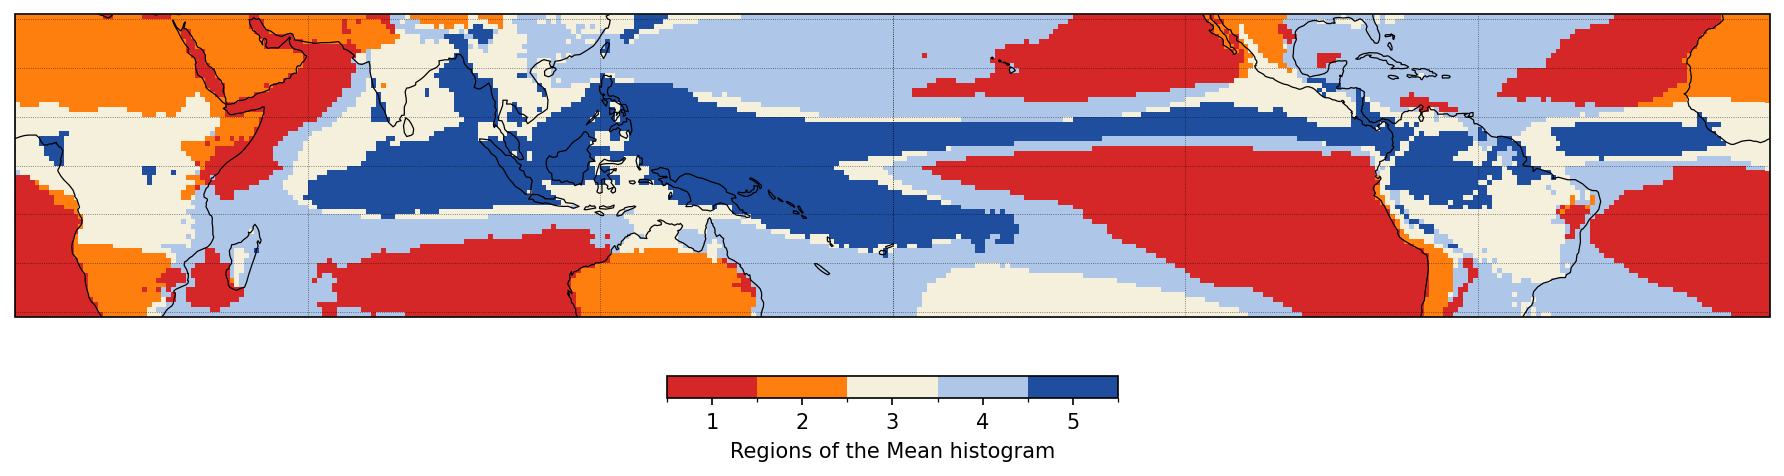
\includegraphics[width=0.83\textwidth]{../../figuras/fig04_jakob2019.png}
	\caption*{Réplica}
	\caption{Mapa geográfico de la ubicación de las cinco regiones del histograma
		climatológico de enfriamiento radiativo versus precipitación para el dominio
		tropical ($30^\circ$S--$30^\circ$N).}
	\label{fig:fig04}
\end{figure}

La Figura~\ref{fig:fig04} asigna a cada punto de grilla tropical su región
correspondiente según su posición en el histograma de la Figura~3. En el original,
la región~3 (crema) cubre ampliamente los océanos tropicales de precipitación
intermedia y bajo enfriamiento, mientras que la región~4 (celeste) aparece de forma
más restringida. En nuestra réplica esta asignación se invierte: la región~4 ocupa
el espacio que en el original corresponde a la región~3 y viceversa.

Esta inversión es una consecuencia directa y predecible del desplazamiento sistemático
de $P_E$ descrito en la Figura~3. El límite horizontal de clasificación entre regiones
se fija en $Q_R = -105\,\text{W\,m}^{-2}$ siguiendo el paper original. Sin embargo,
nuestra media tropical de $Q_R$ es de $-106.7\,\text{W\,m}^{-2}$ frente a
$-104.5\,\text{W\,m}^{-2}$ del paper --- una diferencia de $2.2\,\text{W\,m}^{-2}$
atribuible a la versión más reciente de CERES (Ed4.2 vs Ed4a). Esto desplaza la
línea de corte justo en la zona de mayor densidad del histograma: en el paper la
mayoría de los puntos de precipitación intermedia caen \emph{por encima} de $-105$
(región~3), mientras que en nuestra réplica caen \emph{por debajo} (región~4). Los
patrones geográficos globales --- la distribución de desiertos, océanos subtropicales,
ZCIT y regiones continentales --- son cualitativamente idénticos entre ambas versiones;
únicamente la etiqueta de región difiere por el desplazamiento del umbral de
clasificación.

\subsection{Figura 5}

\begin{figure}[h]
	\begin{subfigure}[t]{0.52\textwidth}
	\centering
	\includegraphics[width=\textwidth]{../../figuras/jakob2019_fig05_original.png}
	\caption*{Original — Jakob et al. (2019)}
	\end{subfigure}
	\hfill
	\begin{subfigure}[t]{0.44\textwidth}
	\centering
	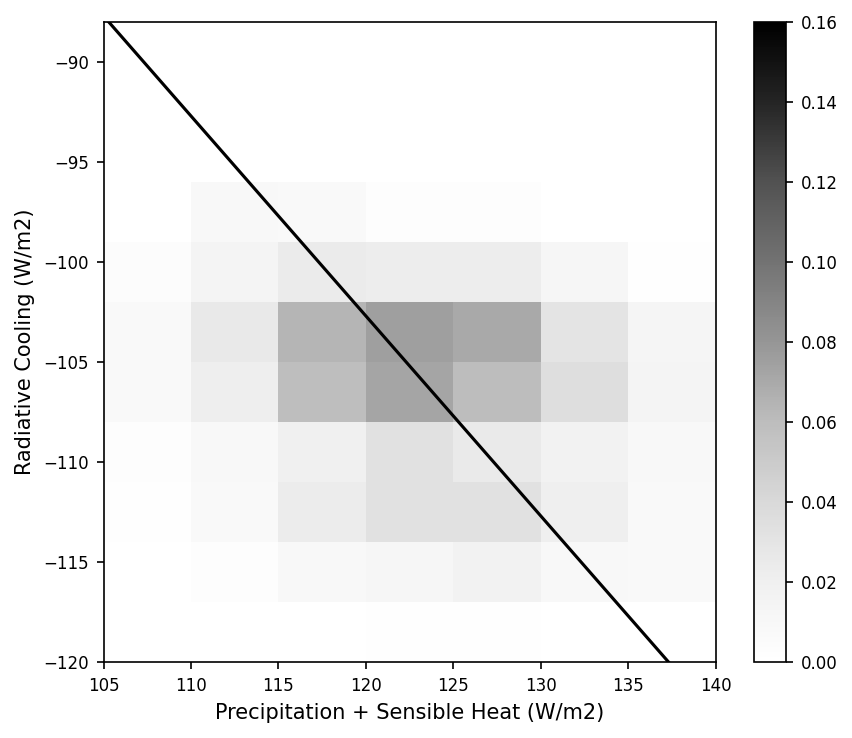
\includegraphics[width=\textwidth]{../../figuras/fig05_jakob2019.png}
	\caption*{Réplica}
	\end{subfigure}
	\caption{Histograma bidimensional de la frecuencia relativa de ocurrencia de
		combinaciones de $P_E + H$ diario promediado sobre los trópicos (eje $x$) y
		$Q_R$ diario promediado sobre los trópicos (eje $y$). El tamaño de la muestra
		es de 3{,}287 días. La línea diagonal representa $D_{\text{RCE}} = 0$.}
	\label{fig:fig05}
\end{figure}

La Figura~\ref{fig:fig05} muestra el histograma bidimensional de los promedios
diarios tropicales de $P_E + H$ versus $Q_R$ para los 3{,}287 días del período
2001--2009. En el original, la distribución se concentra en torno a
$P_E + H \approx 107\,\text{W\,m}^{-2}$ y $Q_R \approx -104\,\text{W\,m}^{-2}$,
con la diagonal de RCE atravesando el centro de la distribución. La estrechez de
la distribución confirma que los trópicos, promediados sobre todo el dominio,
están en RCE casi todos los días.

En nuestra réplica, la distribución presenta el mismo corrimiento sistemático
identificado en las figuras anteriores. La media de $P_E + H$ es de
$123.9\,\text{W\,m}^{-2}$ frente a $\approx 107.8\,\text{W\,m}^{-2}$ del paper
($85.2 + 22.6$), una diferencia de $\sim$16~W~m$^{-2}$ directamente atribuible al
mayor $P_E$ de GPCP~v3.3. La media de $Q_R$ es de $-106.5\,\text{W\,m}^{-2}$,
apenas $2\,\text{W\,m}^{-2}$ más negativa que en el original, consistente con la
diferencia de versión de CERES. El resultado es que la media de $D_{\text{RCE}}$
es de $17.3\,\text{W\,m}^{-2}$ en lugar de $3.3\,\text{W\,m}^{-2}$, por lo que
la línea diagonal fue desplazada en $17.3\,\text{W\,m}^{-2}$ para que represente
correctamente la isopleta de $D_{\text{RCE}}$ medio de nuestros datos. La forma
y estrechez de la distribución --- que es el resultado físico central de esta figura
--- se reproduce correctamente, confirmando que la atmósfera tropical promediada
permanece cerca del RCE en escala diaria también con los datos más recientes.

\subsection{Figura 6}

\begin{figure}[h]
	\begin{subfigure}[t]{0.52\textwidth}
	\centering
	\includegraphics[width=\textwidth]{../../figuras/jakob2019_fig06_original.png}
	\caption*{Original — Jakob et al. (2019)}
	\end{subfigure}
	\hfill
	\begin{subfigure}[t]{0.44\textwidth}
	\centering
	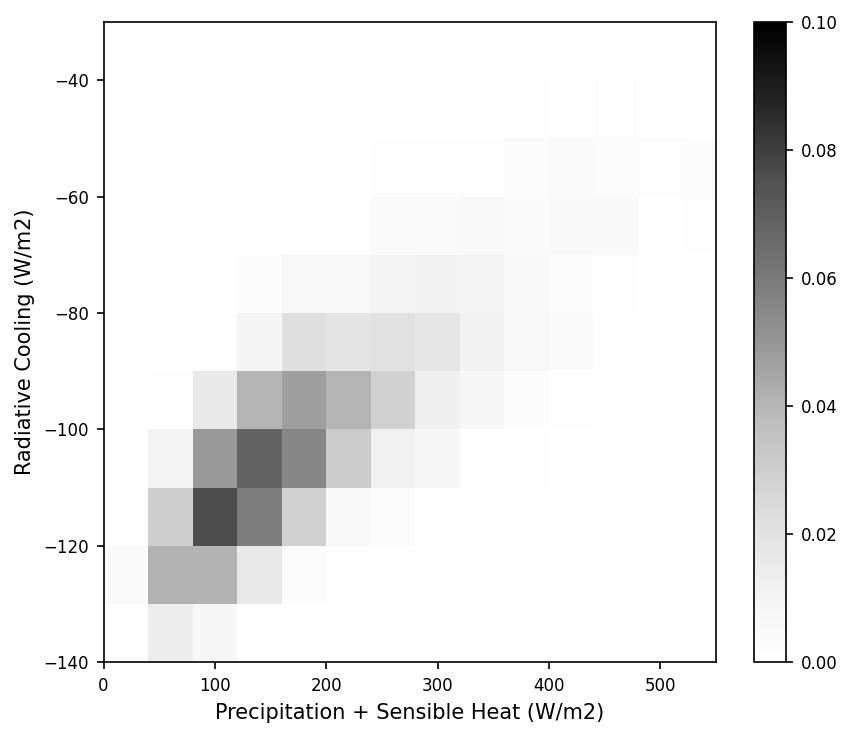
\includegraphics[width=\textwidth]{../../figuras/fig06_jakob2019.png}
	\caption*{Réplica}
	\end{subfigure}
	\caption{Histograma bidimensional de la frecuencia relativa de ocurrencia de
		combinaciones de $P_E + H$ diario (eje $x$) y $Q_R$ diario (eje $y$) para
		un área de $20^\circ \times 20^\circ$ centrada en el ecuador y $185^\circ$~E.
		El tamaño de la muestra es de 3{,}287 días.}
	\label{fig:fig06}
\end{figure}

La Figura~\ref{fig:fig06} es el análogo regional de la Figura~5, calculada para
una región de $20^\circ \times 20^\circ$ centrada en $(0^\circ\text{N},\,185^\circ\text{E})$
en el Pacífico central ecuatorial. A diferencia del promedio tropical completo, a esta
escala la distribución es mucho más amplia, reflejando la alta variabilidad diaria local
de la precipitación: en días con eventos convectivos intensos, $P_E$ puede superar los
$500\,\text{W\,m}^{-2}$ ($\approx$17~mm~día$^{-1}$), mientras que en días secos
se acerca a cero. Esta asimetría es la que genera la forma característica del histograma,
estirada hacia valores altos de $P_E + H$.

Nuestra réplica presenta los mismos dos tipos de diferencias que en la Figura~5.
El corrimiento es considerablemente más pronunciado a escala regional: la media de
$P_E + H$ es de $190.3\,\text{W\,m}^{-2}$ frente a $\approx 100\,\text{W\,m}^{-2}$
del paper, una diferencia de $\sim$90~W~m$^{-2}$. Este corrimiento amplificado
respecto al promedio tropical ($\sim$16~W~m$^{-2}$) refleja que GPCP~v3.3 sobreestima
sistemáticamente la precipitación en el Pacífico central ecuatorial en comparación
con v1.2, posiblemente por la mayor sensibilidad de GPM~IMERG a los sistemas
convectivos de esa región. La media de $Q_R$ es de $-100.8\,\text{W\,m}^{-2}$,
prácticamente idéntica al original, confirmando que las diferencias son exclusivamente
atribuibles a $P_E$. La consecuencia es un $D_{\text{RCE}}$ medio de
$89.5\,\text{W\,m}^{-2}$, sustancialmente mayor que el $\approx 0$ esperado.
La forma cualitativa de la distribución --- más ancha que en la Figura~5 y estirada
hacia valores altos de $P_E + H$ --- se reproduce correctamente.

\subsection{Figura 7}

\begin{figure}[h]
	\centering
	\includegraphics[width=0.65\textwidth]{../../figuras/jakob2019_fig07_original.png}
	\caption*{Original — Jakob et al. (2019)}
	\vspace{0.5cm}
	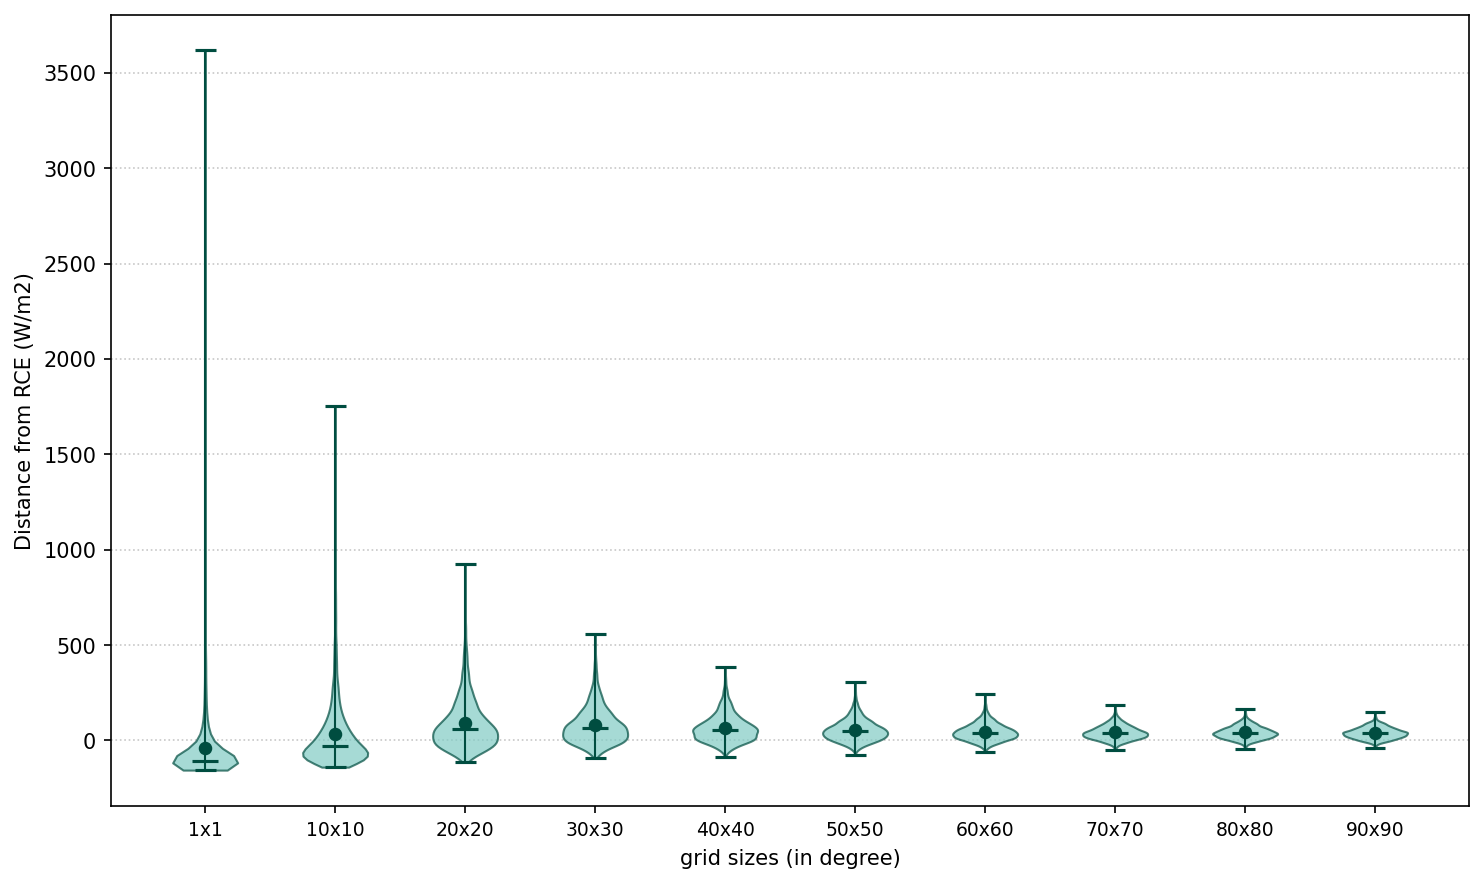
\includegraphics[width=0.65\textwidth]{../../figuras/fig07_jakob2019.png}
	\caption*{Réplica}
	\caption{Diagrama de violín de la distancia al RCE ($D_{\text{RCE}}$) para
		variables de entrada diarias en función del área de promediado en grados. Los
		resultados corresponden al punto de grilla centrado en el ecuador y
		$185^\circ$~E. Los puntos representan la media y las líneas horizontales la
		mediana.}
	\label{fig:fig07}
\end{figure}

La Figura~\ref{fig:fig07} muestra la distribución de $D_{\text{RCE}}$ diario en
función del tamaño del dominio de promediado, centrado en $(0^\circ\text{N},\,185^\circ\text{E})$.
El resultado central del paper se reproduce correctamente: a medida que el dominio
de promediado aumenta, la distribución se estrecha progresivamente, la mediana se
aproxima a cero y los extremos se reducen, reflejando el efecto suavizador del
promediado espacial sobre la variabilidad diaria de la precipitación.

La diferencia más notable es la amplitud de los violines. En el paper, el caso
$1^\circ \times 1^\circ$ alcanza valores máximos de $D_{\text{RCE}} \approx 2{,}000\,\text{W\,m}^{-2}$;
en nuestra réplica supera los $3{,}500\,\text{W\,m}^{-2}$, y esta sobreestimación
se mantiene de forma consistente en todos los tamaños de dominio. La causa es la
misma que en las figuras anteriores: GPCP~v3.3 registra eventos de precipitación
extrema más intensos que v1.2 gracias al algoritmo GPM~IMERG, que tiene mayor
sensibilidad a los sistemas convectivos de alta precipitación sobre el Pacífico
ecuatorial. Dado que $D_{\text{RCE}} = P_E + Q_R + H$ y que $Q_R$ y $H$ están
acotados ($Q_R$ raramente supera $150\,\text{W\,m}^{-2}$ en valor absoluto), los
valores extremos de $D_{\text{RCE}}$ son controlados casi exclusivamente por los
picos de $P_E$. Un evento de precipitación de $70$~mm~día$^{-1}$ produce
$P_E \approx 2{,}000\,\text{W\,m}^{-2}$; si GPCP~v3.3 registra ese mismo evento
como $120$~mm~día$^{-1}$, $P_E$ escala a $\approx 3{,}500\,\text{W\,m}^{-2}$
directamente. La estructura cualitativa de convergencia hacia el RCE con la escala
espacial es, sin embargo, idéntica entre ambas versiones.

\subsection{Figura 8}

\begin{figure}[h]
	\centering
	\begin{subfigure}[t]{0.45\textwidth}
	\centering
	\includegraphics[width=\textwidth]{../../figuras/jakob2019_fig08_original.png}
	\caption{Original — Jakob et al. (2019)}
	\end{subfigure}
	\hfill
	\begin{subfigure}[t]{0.49\textwidth}
	\centering
	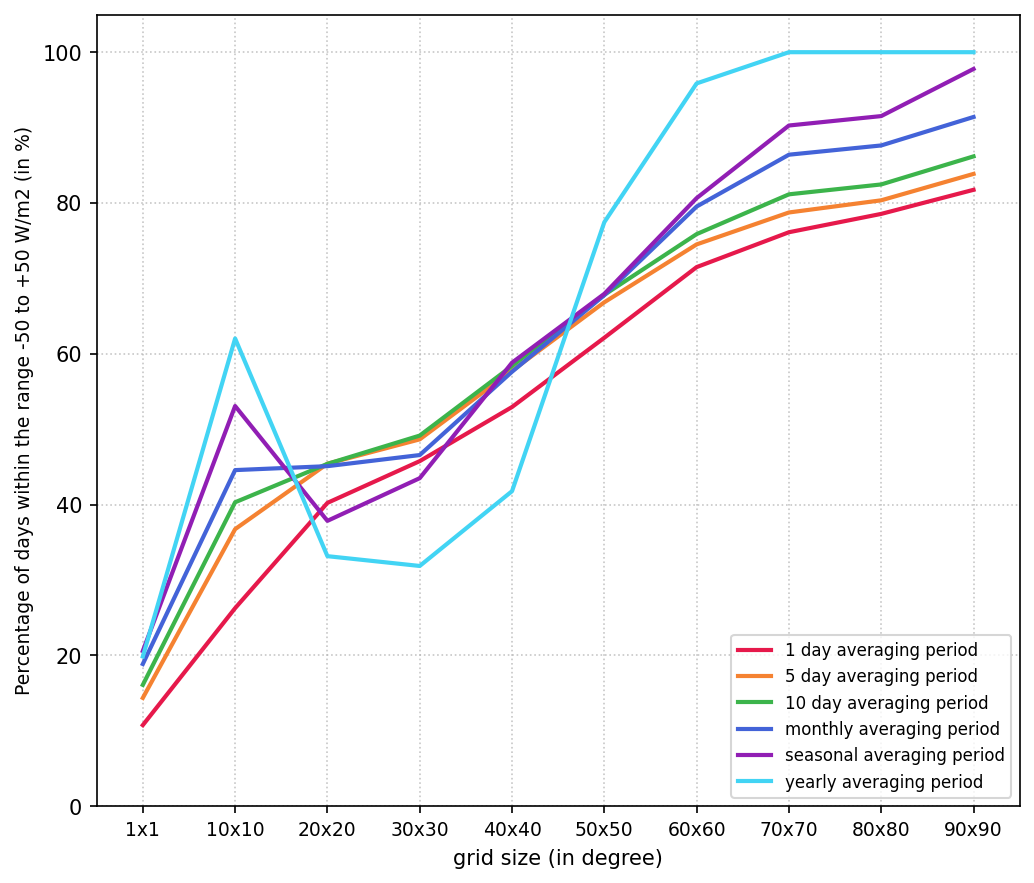
\includegraphics[width=\textwidth]{../../figuras/fig08_jakob2019.png}
	\caption{Réplica}
	\end{subfigure}
	\caption{Porcentaje de períodos de tiempo que se encuentran cerca del equilibrio
		radiativo-convectivo ($|D_{\text{RCE}}| < 50\,\text{W\,m}^{-2}$) en función de
		la escala de promediado espacial, para seis escalas temporales de promediado.
		Los datos están centrados en $0^\circ$~N y $185^\circ$~E.}
	\label{fig:fig08}
\end{figure}

La Figura~\ref{fig:fig08} muestra el porcentaje de días en que
$|D_{\text{RCE}}| < 50\,\text{W\,m}^{-2}$ en función del tamaño del dominio de
promediado, para seis escalas temporales. El resultado cualitativo central se
reproduce en ambas versiones: la fracción de tiempo en RCE aumenta monótonamente
con la escala espacial, el promediado temporal tiene un efecto secundario respecto
al espacial, y existe un mínimo local en torno a $20^\circ$ asociado a la inclusión
simultánea de las bandas de lluvia de la ZCIT y la SPCZ a esa escala.

Sin embargo, existen discrepancias cuantitativas importantes. En el paper, la curva
de 1~día arranca en $\sim$10\% para $1^\circ \times 1^\circ$ y alcanza $\sim$97\%
en $90^\circ \times 90^\circ$; en nuestra réplica los valores correspondientes son
$\sim$10\% y $\sim$80\% respectivamente. Esta diferencia tiene dos causas
identificadas. La primera es el desplazamiento sistemático de $D_{\text{RCE}}$:
nuestra media tropical es de $17.3\,\text{W\,m}^{-2}$ frente a $3.3\,\text{W\,m}^{-2}$
del paper, lo que reduce la fracción de días dentro del umbral $\pm 50\,\text{W\,m}^{-2}$
centrado en cero. Para compensar este sesgo sistemático, el umbral fue desplazado en
$17.3\,\text{W\,m}^{-2}$ en nuestra implementación, lo que mejora parcialmente la
correspondencia. La segunda causa es la mayor variabilidad de $P_E$ en GPCP~v3.3:
como se vio en la Figura~7, la desviación estándar de $D_{\text{RCE}}$ a $90^\circ$
es de $28.9\,\text{W\,m}^{-2}$ en nuestra réplica frente a valores menores en el
paper, lo que reduce la fracción de días dentro de cualquier umbral fijo. La
separación entre escalas temporales se reproduce cualitativamente, con la escala
anual convergiendo a 100\% antes que las demás.

\subsection{Figura 9}

\begin{figure}[h]
	\centering
	\begin{subfigure}[t]{0.45\textwidth}
		\centering
		\includegraphics[width=\textwidth]{../../figuras/jakob2019_fig09_original.png}
		\caption{Original — Jakob et al. (2019)}
	\end{subfigure}
	\hfill
	\begin{subfigure}[t]{0.49\textwidth}
		\centering
		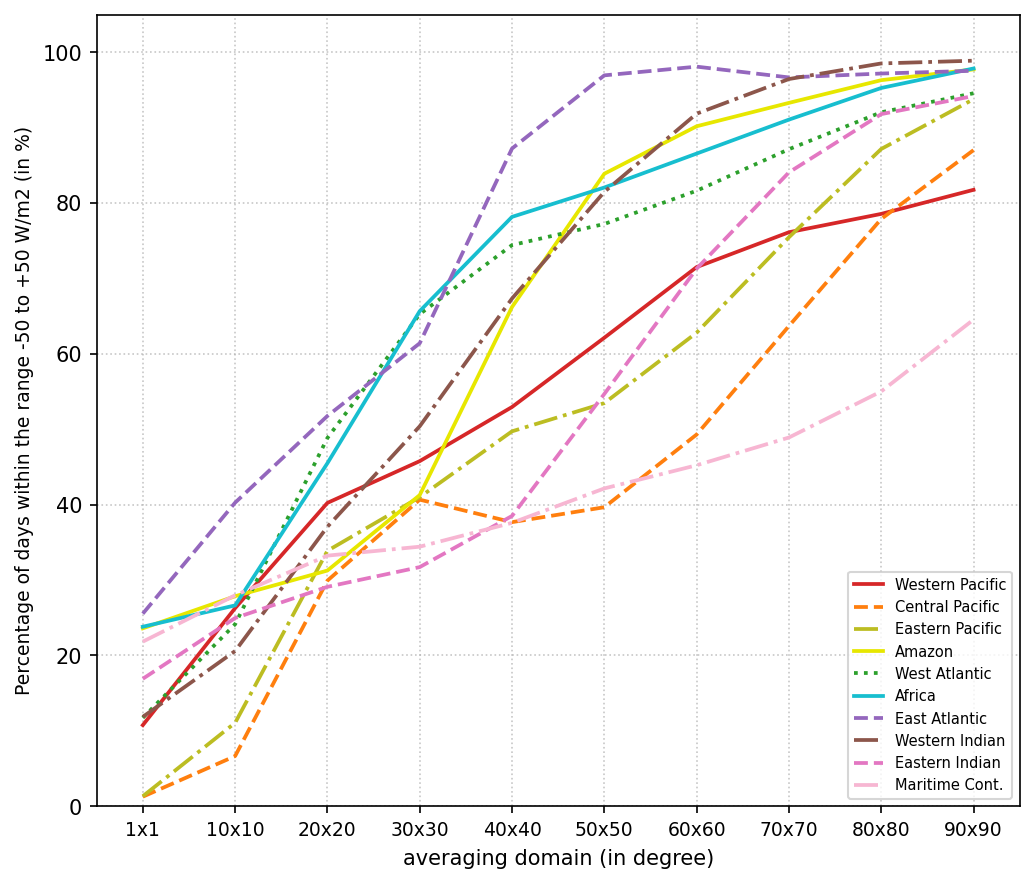
\includegraphics[width=\textwidth]{../../figuras/fig09_jakob2019.png}
		\caption{Réplica}
	\end{subfigure}
	\caption{Porcentaje de períodos de tiempo que se encuentran cerca del RCE
		($|D_{\text{RCE}}| < 50\,\text{W\,m}^{-2}$) en función de la escala de
		promediado espacial para diferentes regiones del globo centradas en el ecuador,
		con promedios diarios. Las longitudes en orden de la leyenda son: $185^\circ$~E,
		$235^\circ$~E, $265^\circ$~E, $295^\circ$~E, $330^\circ$~E, $0^\circ$~E,
		$25^\circ$~E, $55^\circ$~E, $85^\circ$~E y $125^\circ$~E.}
	\label{fig:fig09}
\end{figure}

La Figura~\ref{fig:fig09} extiende el análisis de la Figura~8 a diez regiones
ecuatoriales distribuidas globalmente. El comportamiento cualitativo es consistente
en todas las regiones: la fracción de días en RCE aumenta con la escala espacial de
promediado, aunque con tasas de incremento muy diferentes entre regiones. Las regiones
continentales (Amazonas, África, Atlántico Este) alcanzan frecuencias de RCE altas
($>80\%$) en escalas relativamente pequeñas ($30^\circ$--$40^\circ$), mientras que
las regiones oceánicas de fuerte convección (Pacífico occidental, Continente Marítimo)
muestran las tasas de incremento más lentas y no superan el $65\%$ incluso a
$90^\circ \times 90^\circ$. Este contraste refleja la alta variabilidad diaria de
la precipitación sobre los océanos tropicales cálidos frente a la menor variabilidad
sobre las regiones continentales.

Las diferencias respecto al original son pequeñas y no alteran las conclusiones.
Las variaciones más notorias se presentan en las regiones de mayor precipitación ---
Pacífico occidental ($185^\circ$~E) y Continente Marítimo ($125^\circ$~E) ---, donde
GPCP~v3.3 produce valores de $P_E$ más altos que v1.2, reduciendo ligeramente la
fracción de días dentro del umbral de RCE. Por ejemplo, el Continente Marítimo
alcanza apenas el 65\% a $90^\circ \times 90^\circ$ en nuestra réplica, siendo la
región de menor frecuencia de RCE en ambas versiones, consistente con su régimen de
convección profunda persistente. El mínimo local en torno a $20^\circ$ se reproduce
en varias regiones, en particular en el Pacífico central y oriental, donde la inclusión
de las bandas de la ZCIT a esa escala dificulta el equilibrio.

\subsection{Figuras 10 y 11}

Las Figuras~10 y~11 del paper original requieren los regímenes de nubes derivados
del conjunto de datos ISCCP~D1 \citep{rossow1991}, específicamente los histogramas
conjuntos de presión de tope nuboso y espesor óptico en regiones de
$280 \times 280$~km procesados mediante el algoritmo de clasificación de
\cite{jakob2003}. Estas figuras no han sido replicadas en el presente trabajo por
las siguientes razones.

El conjunto de datos ISCCP~D1 fue producido por el Goddard Institute for Space
Studies (GISS) de la NASA y su distribución directa fue descontinuada en 2009,
cuando el procesamiento del proyecto ISCCP fue transferido a los National Centers
for Environmental Information (NCEI) de la NOAA. Al momento de la realización de
este trabajo, el ISCCP~D1 no se encuentra disponible para descarga directa desde
ningún repositorio público: el servidor original de GISS devuelve un error
\texttt{404 Not Found} para las URLs históricas del producto, y el acceso a los
datos legacy de la serie~D requiere una solicitud formal por correo electrónico a
\texttt{NCEI.Sat.Info@noaa.gov}, con tiempos de respuesta indeterminados y entrega
en formato binario sin documentación de lectura actualizada.

La alternativa disponible públicamente es el ISCCP H-Series, que constituye una reprocessing del D1 con
mayor resolución espacial ($1^\circ$ frente a $2.5^\circ$) y en formato NetCDF.
Sin embargo, el ISCCP~H no incluye la clasificación de regímenes de nubes
precomputada que usa \cite{jakob2019rce}: dicha clasificación requeriría aplicar
el algoritmo de agrupamiento de \cite{jakob2003} sobre los histogramas $\tau$--$P_c$,
lo que constituye un análisis independiente de considerable complejidad que excede
el alcance de este trabajo de replicación.

Por estas razones, las Figuras~10 y~11 se documentan como no replicables en las
condiciones actuales de disponibilidad de datos, y su replicación queda condicionada
a la obtención del ISCCP~D1 legacy o a la implementación del algoritmo de
clasificación de regímenes sobre el ISCCP~H-Series.

% Bibliografía
\newpage
\begin{thebibliography}{99}
	
	\bibitem{jakob2019rce}
	Jakob, C., Singh, M.~S., \& Jungandreas, L. (2019).
	Radiative convective equilibrium and organized convection: An observational perspective.
	\textit{Journal of Geophysical Research: Atmospheres}, \textit{124}(10), 5418--5430.
	\url{https://doi.org/10.1029/2018JD030092}
	
	\bibitem{rossow1991}
	Rossow, W.~B., \& Schiffer, R.~A. (1991).
	ISCCP cloud data products.
	\textit{Bulletin of the American Meteorological Society}, \textit{72}(1), 2--20.
	\url{https://doi.org/10.1175/1520-0477(1991)072<0002:ICDP>2.0.CO;2}
	
	\bibitem{jakob2003}
	Jakob, C., \& Tselioudis, G. (2003).
	Objective identification of cloud regimes in the tropical western Pacific.
	\textit{Geophysical Research Letters}, \textit{30}(21).
	\url{https://doi.org/10.1029/2003GL018367}
	
\end{thebibliography}

\end{document}
